\documentclass{article}
\usepackage[utf8]{inputenc}

\newenvironment{changemargin}[2]{%
\begin{list}{}{%
\setlength{\topsep}{0pt}%
\setlength{\leftmargin}{#1}%
\setlength{\rightmargin}{#2}%
\setlength{\listparindent}{\parindent}%
\setlength{\itemindent}{\parindent}%
\setlength{\parsep}{\parskip}%
}%
\item[]}{\end{list}}

\usepackage{geometry}
\newgeometry{left=3cm,top=2cm}

\usepackage[pdftex]{hyperref}
\usepackage{graphicx,float}
\usepackage{parskip}
\usepackage{caption}
\usepackage{amsmath}
\usepackage{listings}
\usepackage{xcolor}
\usepackage{multicol}
\usepackage[portuguese]{babel}

\usepackage{listings}     
\usepackage{lstautogobble}  % Fix relative indenting
\usepackage{color}          % Code coloring
\usepackage{zi4}            % Nice font

\definecolor{bluekeywords}{rgb}{0.13, 0.13, 1}
\definecolor{greencomments}{rgb}{0, 0.5, 0}
\definecolor{redstrings}{rgb}{0.9, 0, 0}
\definecolor{graynumbers}{rgb}{0.5, 0.5, 0.5}

\usepackage{listings}
\lstset{
    autogobble,
    columns=fullflexible,
    showspaces=false,
    showtabs=false,
    breaklines=true,
    showstringspaces=false,
    breakatwhitespace=true,
    escapeinside={(@}{@)},
    commentstyle=\color{greencomments},
    keywordstyle=\color{bluekeywords},
    stringstyle=\color{redstrings},
    numberstyle=\color{graynumbers},
    basicstyle=\ttfamily\footnotesize,
    frame=l,
    framesep=12pt,
    xleftmargin=12pt,
    tabsize=4,
    captionpos=b
}

\title{\textbf{Artigo - Modelagem de Fenômenos Biológicos}}
\author{\textbf{Raphael Levy e Erick Brito}}
\date{}

\begin{document}

\maketitle
\\
\begin{center}
    \textbf{\Large{Resumo}}
    \\\\Nesse artigo iremos analisar o comportamento dinâmico de um quimiostato baseado em um modelo com equação de Monod, um tipo de modelo para o crescimento de microrganismos desenvolvido por Jacques Monod.
\end{center}
\\\\
\begin{center}
    \textbf{\Large{Abstract}}
    \\\\In this article we will analyze the dynamic behavior of a chemostat based on a model with Monod equation, a type of model for the growth of microorganisms developed by Jacques Monod. 
\end{center}
\\\\
 
\\\\
\textbf{\Large{Introdução}}
\\\\Como forma de avaliação para o curso de Modelagem de Fenômenos Biológicos, decidimos analisar modelos de crescimento de microrganismos. Mais precisamente, escolhemos analisar o modelo de um \textbf{quimiostato} ($\textbf{chemostat}$, em inglês). O quimiostato é um tipo de biorreator, um equipamento laboratorial inventado em 1950 quase que simultaneamente por Jacques Monod e Aaron Novick $\&$ Leo Szilard, em que um meio de cultura ``fresco" (substrato) é continuamente adicionado, enquanto que o meio anterior com o substrato ``restante" é continuamente removido na mesma taxa, mantendo o volume constante, e é usado para controlar a taxa de crescimento dos microganismos presentes $^{[1]}$. Além disso, é possível também regular níveis de pH, temperatura e oxigenação $^{[2]}$. O nome em si significa ``[ambiente] químico estático".

\begin{figure}[H]
        \centering
        \hbox{\hspace{7.0em} 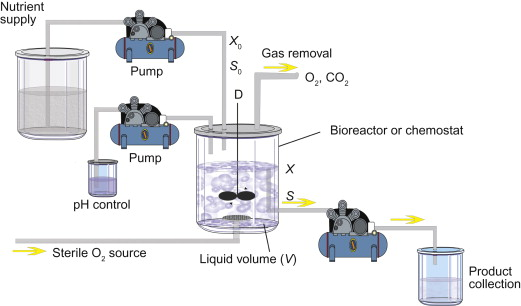
\includegraphics[scale=1.0] {Funcionamento_Quimiostato.jpg}} 
        \caption*{Funcionamento de um quimiostato $^{[2]}$}
\end{figure}
\\\\Um exemplo de funcionamento de um quimiostato pode ser encontrado em $^{[4]}$.
\\\\Para análise de competições entre organismos no quimiostato, são utilizados modelos matemáticos baseados em equações diferenciais, com algumas pequenas variações dependendo do estudo feito. Originalmente, muitos modelos de quimiostato assumiam que o coeficiente de rendimento de biomassa era constante, mas observações experimentais indicavam que um rendimento constante não poderia explicar o comportamento oscilatório presente no quimiostato, como indicado por Rana e Kulsum $^{[5]}$, o que ocorre, em particular, com células de $Saccharomyces cervisae$ e de fitoplâncton $^{[6]}$, organismos estudados por Porro $et \ al.$, que estudavam a aparição espontânea de oscilações em condições aeróbicas em culturas de levedura $^{[7]}$, e por Nisbet e Gurney, que estudavam a resposta de populações a flutuações ambientais contínuas $^{[8]}$. 
\\\\Foi sugerido então que se usasse um coeficiente linear, com um ciclo limitante, e posteriormente Huang $^{[9]}$ e Pilyugin e Waltman $^{[10]}$ desenvolveram modelos com um rendimento variável em vários ciclos, porém esses modelos ainda consideravam apenas o estudo de um único microrganismo por vez. Assim, em 1999, um modelo tridimensional, desenvolvido por Song G. e X. Li $^{[11]}$, que utilizava dois microrganismos, com funções de reações de tipo Monod \footnote{Uma equação Monod é um tipo de modelo matemático para o crescimento de microrganismos, desenvolvido por Monod, relacionando a taxa de crescimento dos microrganismos com a concentração de meio nutritivo limitado em um ambiente aquoso. A equação é dada por:
\begin{center}
    $\mu = \mu_{max} \frac{[S]}{K_s + [S]}$
\end{center}
Onde $\mu$ é a taxa de crescimento do microrganismo em estudo, $\mu_{max}$ é a taxa máxima de seu crescimento, $[S]$ é a concentração do substrato limitante para o crescimento $S$ e $K_s$ é o valor de $[S]$ quando $ \mu/\mu_{max} = 0.5$ ($K_s$ é a ``constante da meia-velocidade").\\\\} $^{[12]}$ e coeficientes de rendimento assumidos como uma função linear da concentração de nutriente, conseguiu estabilidade.
\\\\Em contrapartida, outros estudos indicam que a taxa de crescimento não se ajusta de forma imediata às mudanças no estado estacionário da entrada de substrato ou na taxa de diluição, como previsto por uma equação de Monod, mas na verdade passa por um ``atraso" em resposta às alterações na cultura, que é conhecido como um fenômeno inerte ou efeito de histerese \footnote{Tendência de um sistema de conservar suas propriedades na ausência de um estímulo que as gerou $^{[14]}$, retardo de um efeito quando forças agindo sobre o corpo ou sistema são alteradas $^{[15]}$.}. Assim, foram desenvolvidos modelos que levam em consideração uma equação dinâmica que relaciona a taxa de crescimento específica à concentração de substrato limitante no quimiostato $^{[13]}$. Nesse artigo íamos estudar o modelo dinâmico proposto por Young $et \ al.$, porém como esse modelo faz uso de equações com atraso, decidimos modelar as análises usando o modelo ``simples" de Monod. As equações abaixo vieram ambas dos estudos de  Young $et \ al. $ $^{[13]}$ 
\\\\
\textbf{\Large{Metodologia}}
\\\\O modelo que utilizaremos será o modelo de Monod:
\begin{center}
    $(dX/dt) &= \mu X-DX$     
  \\$(dS/dt) &= DS_f-DS-(\mu X/Y)$
  \\$\mu &= \mu_{max}S/(K_s+S)$
  \\$D \leq \mu_{max}S_f/(K_s + S_f)$
\end{center}
\\\\Onde:

\begin{itemize}
\item $X$ = Concentração de massa celular (Massa/Volume)
\item $S$ = Limite de concentração de saída do substrato (Massa/Volume)
\item $S_f$ = Limite de concentração de entrada do substrato (Massa/Volume)
\item $D$ = Taxa de diluição (1/Tempo)
\item $\mu$ = Taxa de crescimento específica (1/Tempo)
\item $\mu_{max}$ = Máxima taxa de crescimento específica (1/Tempo)
\item $Y$ = Coeficiente de rendimento (Massa celular/Massa do substrato limitante)
\item $K_s$ = Constante de saturação (Massa/Volume)
\end{itemize}
\\\\Analisando as equações (1), (2) e (3) dimensionalmente temos:
\begin{itemize}
    \item A taxa $\frac{dX}{dt}$ do lado esquerdo de (1) tem as unidades $\frac{Massa/Volume}{Tempo} = \frac{Massa}{Volume \cdot Tempo}$. Observando o lado direito, $\mu X - DX$, e substituindo pelas unidades teremos: 
    $$\frac{Massa}{Volume} \cdot \frac{1}{Tempo} - \frac{1}{Tempo} \cdot \frac{Massa}{Volume}$$
    $$= \frac{Massa}{Tempo \cdot Volume}$$
    Pelo fato de terem as mesmas unidades podemos somá-las, então a unidade do lado direito será $\frac{Massa}{Volume \cdot Tempo}$.
    \item Análogo ao lado esquerdo de (1), o lado esquerdo de (2) tem a unidade $\frac{Massa}{Volume \cdot Tempo}$. Substituindo pelas unidades do lado direito teremos:
    $$\frac{1}{Tempo} \cdot \frac{Massa}{Volume} - \frac{1}{Tempo} \cdot \frac{Massa}{Volume} - \frac{1}{Tempo} \cdot \frac{\frac{Massa}{Volume}}{\frac{Massa}{Massa}} $$
    $$= \frac{Massa}{Tempo \cdot Volume} - \frac{Massa}{Tempo \cdot Volume} - \frac{Massa}{Tempo \cdot Volume}$$
    $$= \frac{Massa}{Tempo \cdot Volume} $$
    Assim, a equação (2) também possui as dimensões condizentes.
    \item Na equação (3), temos do lado esquerdo $\mu$, que tem unidade $\frac{1}{Tempo}$. Substituindo pelas unidades no lado direito teremos:
    $$\frac{1}{Tempo} \cdot \left(\frac{\frac{Massa}{Volume}}{\frac{Massa}{Volume} + \frac{Massa}{Volume}}\right)$$
    $$= \frac{1}{Tempo}$$
    Portanto, (3) também é válida quanto às unidades.
    
\end{itemize}
\\\\Esses dados podem ser encontrados em $^{[13]}$. O modelo acima pode ser modificado para considerar coeficientes de rendimento variantes e inibição de substrato, mas o modelo Monod continua falho na predição de comportamento dinâmico em quimiostatos experimentais, o que foi mostrado nos estudos de Mateles et al em $^{[16]}$ e Storer e Gaudy em $^{[17]}$. Esses estudos mostram que a taxa específica de crescimento de células bacterianas não se ajustam instantaneamente às mudanças em $S$ ou perturbações nos valores estáveis de $D$ e de $S_o$.
\\\\Em resumo, embora vários experimentos em quimiostatos distintos indiquem que a taxa de crescimento específica pode responder de forma instantânea para uma pequena quantidade de mudanças no limite de concentração de saída do substrato, alterações mais rápidas levam a ajustes mais lentos e um atraso na taxa de crescimento, consequentemente desenvolvendo um efeito de histerese, algo que não é previsto no modelo Monod.
\\\\Com tantas melhorias possíveis descritas, a equação de Monod deveria ser utilizada para predizer o comportamento dinâmico de um quimiostato? Podemos responder essa questão considerando a origem da da mesma e pensando sobre o seu real significado. O desenvolvimento da equação de Monod e a determinação experimental de $\hat{\mu}$ e $K_s$ têm sido discutidos em muitos trabalhos, o mais notável Herbert \textit{et al} $^{[19]}$. Independentemente de $\hat{\mu}$ e $K_s$ serem determinados a partir de cultura em lotes ou a partir de dados de cultura contínua em estado estacionário, a equação de Monod aplicada a uma cultura contínua define uma série de estados estacionários ou condições de equilíbrio que uma determinada cultura pode operar. Em cada ponto da curva Monod, todos os mecanismos envolvidos no crescimento e reprodução, como transferência de massa através da membrana citoplasmática, formação de monômeros bioquímicos e a síntese macromolecular subsequente, estabeleceram taxas constantes que, por sua vez, se manifestam de forma estável em uma taxa de crescimento específica. 
\\\\
\textbf{\Large{Resultados}}
\\\\As análises gráficas realizadas sobre o modelo de Monod podem ser encontradas nos arquivos
\\ \href{https://github.com/RaphaLevy/Artigo_Fenomenos_Biologicos/blob/main/code/Integracao_Numerica.ipynb}{code/Integracao\_Numerica.ipynb} e \href{https://github.com/RaphaLevy/Artigo_Fenomenos_Biologicos/blob/main/code/Solucao_Analitica.ipynb}{code/Solucao\_Analitica.ipynb}, no repositório da avaliação. Usando o modelo indicado pelas equações (1), (2) e (3), buscamos alguns artigos (ver $^{[20]}$ e $^{[21]}$) que também utilizassem o modelo de Monod para um biorreator contínuo, para podermos utilizar valores iniciais para os parâmetros de forma que faça sentido para o cálculo do modelo, ou seja, garantir que, selecionando valores arbitrariamente, não danificaríamos a modelagem apenas por escolher valores que a equação não poderia suportar. 
\\\\Assim, para que pudéssemos elaborar uma modelagem gráfica, fizemos primeiro uma análise mais ``direta", baseada no notebook sobre estabilidade de equilíbrios elaborada pelo professor $^{[22]}$.
\\\\Usando os valores $dX/dt$ e $dS/dt$ para encontrar os equilíbrios:
\begin{figure}[H]
        \centering
        \hbox{\hspace{7.0em} 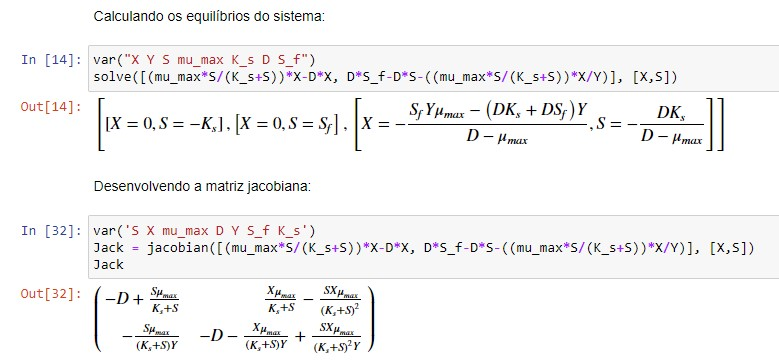
\includegraphics[scale=0.5] {Equilibrios.jpg}} 
\end{figure}
\\\\Tendo os diferentes equilíbrios, podemos começar a plotagem dos gráficos. É preciso notar no entanto que, em geral, o sistema irá sempre convergir para o equilíbrio em $X = Y(S_f- K_sD/(\mu_{max}-D)), S = K_sD/(\mu_{max}-D)$, e só irá convergir para $X = 0, S=S_f$ quando $X_0=0$. Já que $S$ (limite de concentração de substrato de saída) e $K_s$ (constante de saturação) devem ser positivos, não conseguimos identificar um caso com equilíbrio em $X = 0, S=-K_s$.

\newpage
\\\\Agora que já sabemos as equações do equilíbrio, vamos fazer as análises gráficas, começando pela integração numérica de Runge-Kutta:
\begin{figure}[H]
        \centering
        \hbox{\hspace{1.0em} 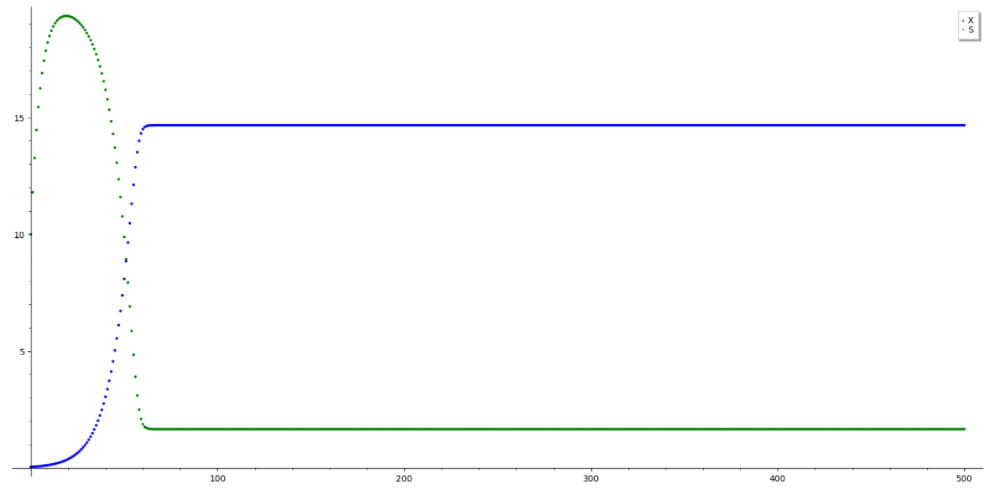
\includegraphics[scale=0.5]{Modelo_1.png}} 
        \caption*{Parâmetros originais (1)}
\end{figure}
\vspace{-7mm}
\begin{itemize}
\begin{multicols}{4}
    \item $\mu_{max} = 1.6$ 
    \item $K_s = 1.0$ 
\columnbreak     
    \item $Y = 0.8$ 
    \item $S_f = 20$ 
\columnbreak    
    \item $D = 1.0$ 
    \item $X_0 = 0.05$ 
\columnbreak     
    \item $S_0 = 10.0$ 
    \item $\mu = 1.0$
\end{multicols}
\end{itemize}
%FEITO 1
\begin{figure}[H]
        \centering
        \hbox{\hspace{1.0em} 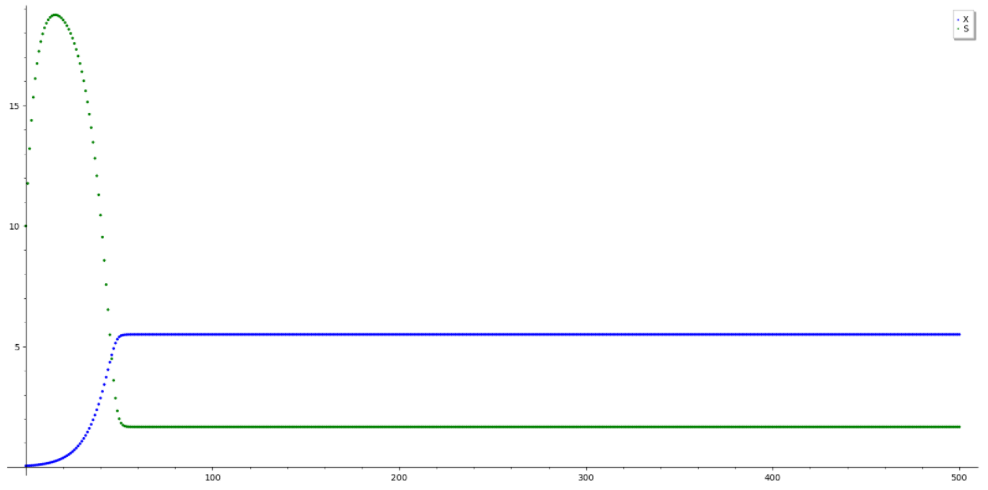
\includegraphics[scale=0.5]{Modelo_2.png}} 
        \caption*{Diminuindo o coeficiente de rendimento (2)}
\end{figure}
\vspace{-7mm}
\begin{itemize}
\begin{multicols}{4}
    \item $\mu_{max} = 1.6$ 
    \item $K_s = 1.0$ 
\columnbreak     
    \item $Y = 0.3$ 
    \item $S_f = 20$ 
\columnbreak    
    \item $D = 1.0$ 
    \item $X_0 = 0.05$ 
\columnbreak     
    \item $S_0 = 10.0$ 
    \item $\mu = 1.0$
\end{multicols}
\end{itemize}   
%FEITO 2 
\begin{figure}[H]
        \centering
        \hbox{\hspace{1.0em} 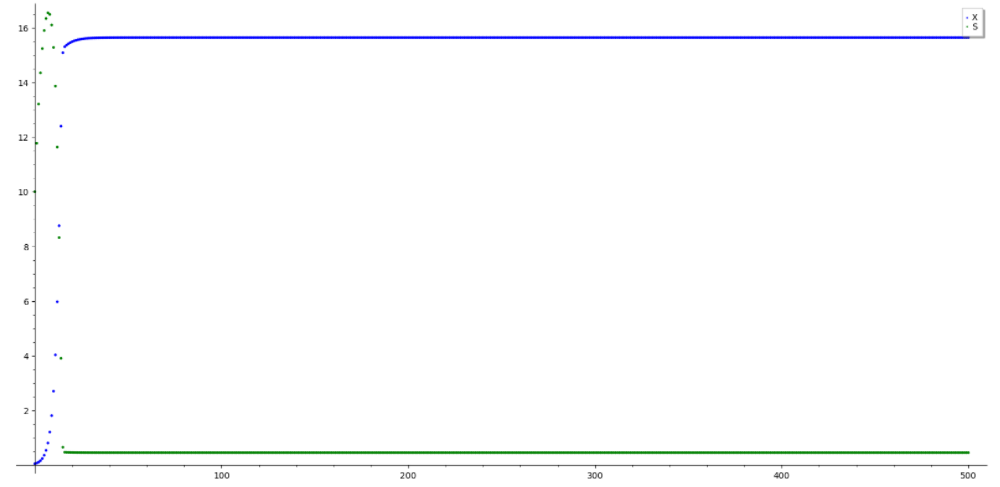
\includegraphics[scale=0.5]{Modelo_3.png}} 
        \caption*{Dobrando a taxa máxima de crescimento (3)}
\end{figure}
\vspace{-7mm}
\begin{itemize}
\begin{multicols}{4}
    \item $\mu_{max} = 3.2$ 
    \item $K_s = 1.0$ 
\columnbreak     
    \item $Y = 0.8$ 
    \item $S_f = 20$ 
\columnbreak    
    \item $D = 1.0$ 
    \item $X_0 = 0.05$ 
\columnbreak     
    \item $S_0 = 10.0$ 
    \item $\mu = 1.0$
\end{multicols}
\end{itemize} 
%FEITO 3
\begin{figure}[H]
        \centering
        \hbox{\hspace{1.0em} 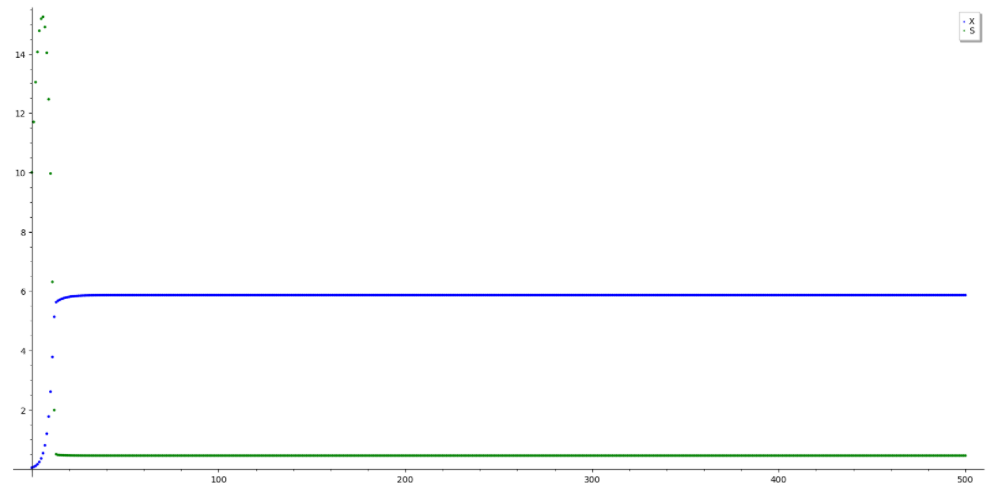
\includegraphics[scale=0.5]{Modelo_4.png}} 
        \caption*{Dobrando a taxa máxima de crescimento e diminuindo o coeficiente de rendimento (4)}
\end{figure}
\vspace{-7mm}
\begin{itemize}
\begin{multicols}{4}
    \item $\mu_{max} = 3.2$ 
    \item $K_s = 1.0$ 
\columnbreak    
    \item $Y = 0.3$ 
    \item $S_f = 20$ 
\columnbreak    
    \item $D = 1.0$ 
    \item $X_0 = 0.05$ 
\columnbreak    
    \item $S_0 = 10.0$ 
    \item $\mu = 1.0$
\end{multicols}
\end{itemize} 
%FEITO 4 
\begin{figure}[H]
        \centering
        \hbox{\hspace{1.0em} 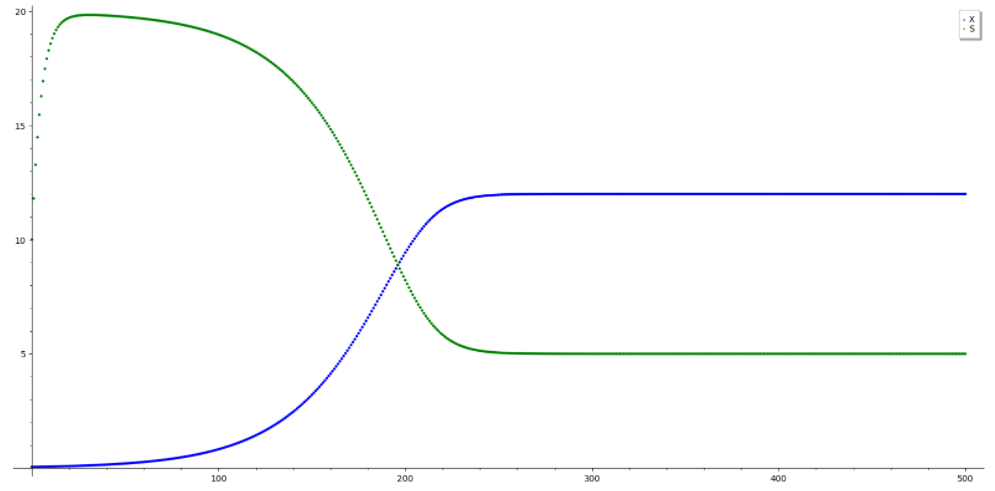
\includegraphics[scale=0.5]{Modelo_5_New.png}} 
        \caption*{Diminuindo a taxa máxima de crescimento (5)}
\end{figure}
\vspace{-7mm}
\begin{itemize}
\begin{multicols}{4}
    \item $\mu_{max} = 1.2$ 
    \item $K_s = 1.0$ 
\columnbreak    
    \item $Y = 0.8$ 
    \item $S_f = 20$ 
\columnbreak    
    \item $D = 1.0$ 
    \item $X_0 = 0.05$ 
\columnbreak    
    \item $S_0 = 10.0$ 
    \item $\mu = 1.0$
\end{multicols}
\end{itemize} 
%FEITO 5 
\begin{figure}[H]
        \centering
        \hbox{\hspace{1.0em} 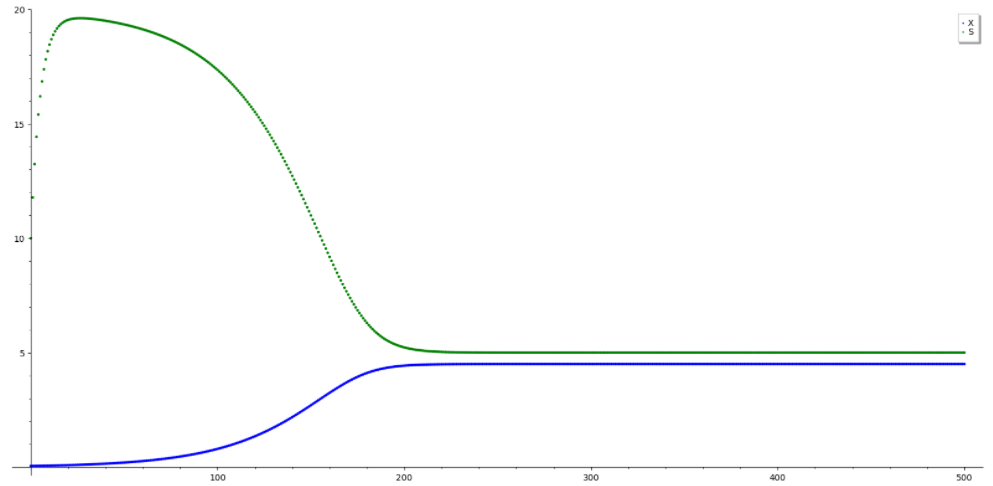
\includegraphics[scale=0.5]{Modelo_6_New.png}} 
        \caption*{Diminuindo a taxa máxima de crescimento e diminuindo o coeficiente de rendimento (6)}
\end{figure}
\vspace{-7mm}
\begin{itemize}
\begin{multicols}{4}
    \item $\mu_{max} = 1.2$ 
    \item $K_s = 1.0$ 
\columnbreak    
    \item $Y = 0.3$ 
    \item $S_f = 20$ 
\columnbreak    
    \item $D = 1.0$ 
    \item $X_0 = 0.05$ 
\columnbreak    
    \item $S_0 = 10.0$ 
    \item $\mu = 1.0$
\end{multicols}
\end{itemize} 
%FEITO 6
\begin{figure}[H]
        \centering
        \hbox{\hspace{1.0em} 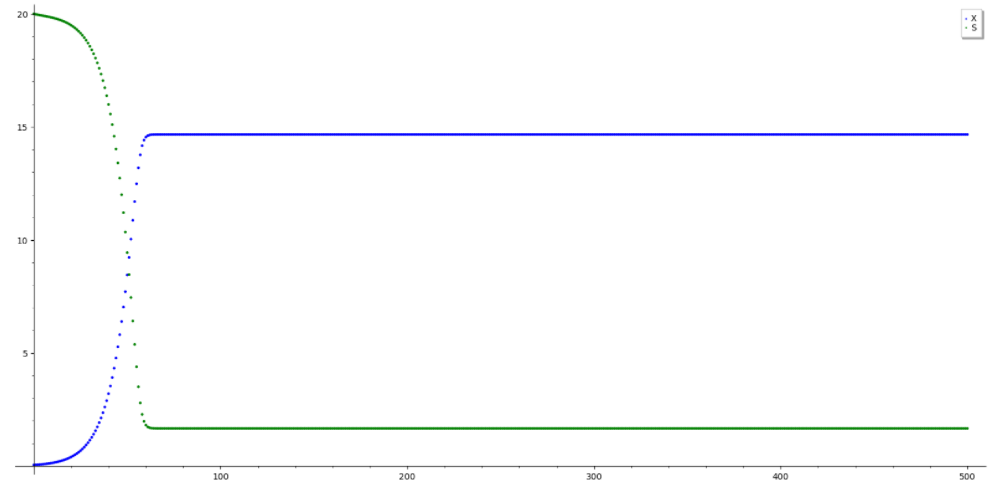
\includegraphics[scale=0.5]{Modelo_7.png}} 
        \caption*{Dobrando o limite de concentração de saída do substrato (7)}
\end{figure}
\vspace{-7mm}
\begin{itemize}
\begin{multicols}{4}
    \item $\mu_{max} = 1.6$ 
    \item $K_s = 1.0$ 
\columnbreak    
    \item $Y = 0.8$ 
    \item $S_f = 20$ 
\columnbreak    
    \item $D = 1.0$ 
    \item $X_0 = 0.05$ 
\columnbreak    
    \item $S_0 = 20.0$ 
    \item $\mu = 1.0$
\end{multicols}
\end{itemize} 
%NÃO DÁ PRA FAZER
\begin{figure}[H]
        \centering
        \hbox{\hspace{1.0em} 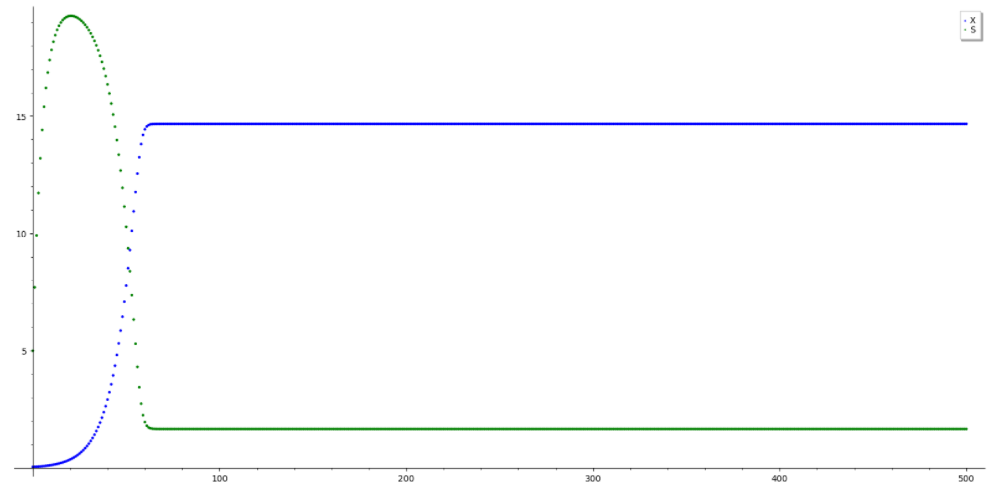
\includegraphics[scale=0.5]{Modelo_8.png}} 
        \caption*{Diminuindo o limite de concentração de saída do substrato pela metade (8)}
\end{figure}
\vspace{-7mm}
\begin{itemize}
\begin{multicols}{4}
    \item $\mu_{max} = 1.6$ 
    \item $K_s = 1.0$ 
\columnbreak    
    \item $Y = 0.8$ 
    \item $S_f = 20$ 
\columnbreak    
    \item $D = 1.0$ 
    \item $X_0 = 0.05$ 
\columnbreak    
    \item $S_0 = 5.0$ 
    \item $\mu = 1.0$
\end{multicols}
\end{itemize} 
%NÃO DÁ PRA FAZER
\begin{figure}[H]
        \centering
        \hbox{\hspace{1.0em} 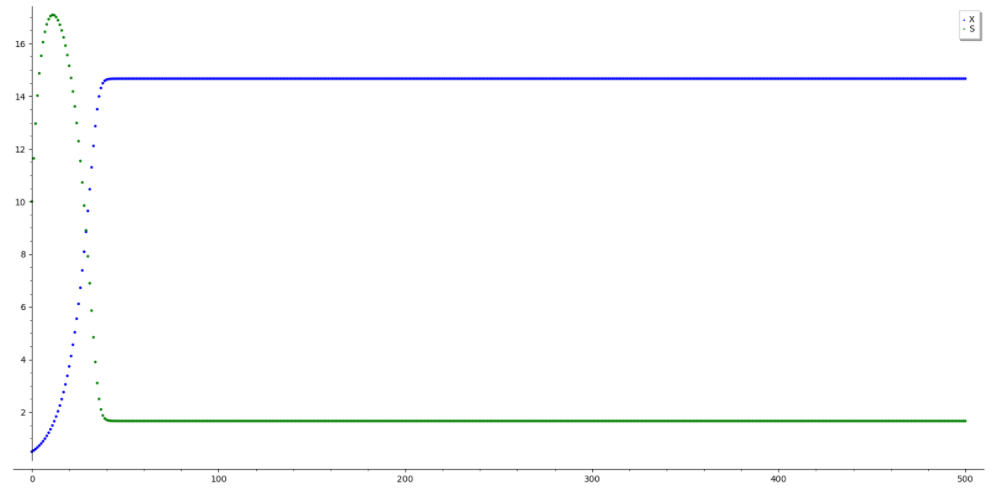
\includegraphics[scale=0.5]{Modelo_9.png}} 
        \caption*{Aumentando a concentração de massa celular em 10 vezes (9)}
\end{figure}
\vspace{-7mm}
\begin{itemize}
\begin{multicols}{4}
    \item $\mu_{max} = 1.6$ 
    \item $K_s = 1.0$ 
\columnbreak    
    \item $Y = 0.8$ 
    \item $S_f = 20$ 
\columnbreak    
    \item $D = 1.0$ 
    \item $X_0 = 0.5$ 
\columnbreak    
    \item $S_0 = 10.0$ 
    \item $\mu = 1.0$
\end{multicols}
\end{itemize} 
%NÃO DÁ PRA FAZER
\begin{figure}[H]
        \centering
        \hbox{\hspace{1.0em} 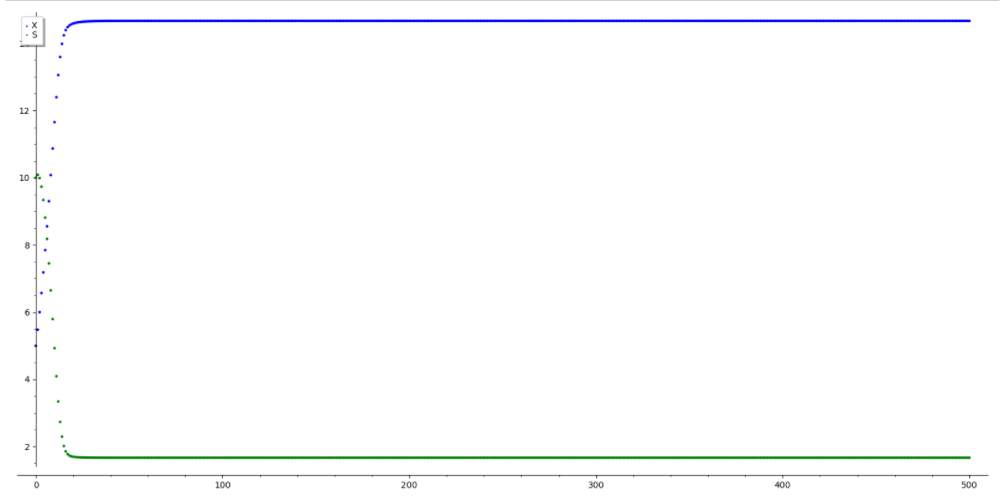
\includegraphics[scale=0.5]{Modelo_10.png}} 
        \caption*{Aumentando a concentração de massa celular em 100 vezes (10)}
\end{figure}
\vspace{-7mm}
\begin{itemize}
\begin{multicols}{4}
    \item $\mu_{max} = 1.6$ 
    \item $K_s = 1.0$ 
\columnbreak    
    \item $Y = 0.8$ 
    \item $S_f = 20$ 
\columnbreak    
    \item $D = 1.0$ 
    \item $X_0 = 5.0$ 
\columnbreak    
    \item $S_0 = 10.0$ 
    \item $\mu = 1.0$
\end{multicols}
\end{itemize}
%NÃO DÁ PRA FAZER
\begin{figure}[H]
        \centering
        \hbox{\hspace{1.0em} 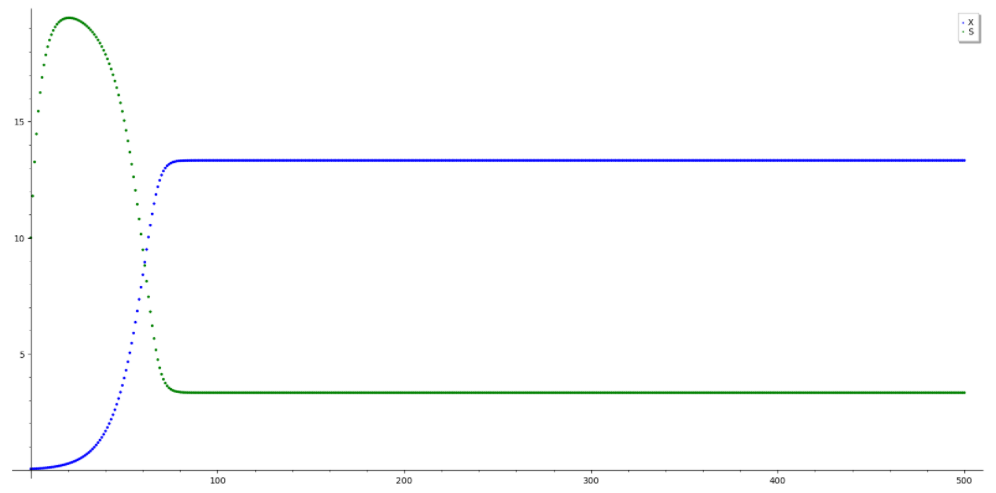
\includegraphics[scale=0.5]{Modelo_11.png}} 
        \caption*{Dobrando a constante de saturação (11)}
\end{figure}
\vspace{-7mm}
\begin{itemize}
\begin{multicols}{4}
    \item $\mu_{max} = 1.6$ 
    \item $K_s = 2.0$ 
\columnbreak    
    \item $Y = 0.8$ 
    \item $S_f = 20$ 
\columnbreak    
    \item $D = 1.0$ 
    \item $X_0 = 0.05$ 
\columnbreak    
    \item $S_0 = 10.0$ 
    \item $\mu = 1.0$
\end{multicols}
\end{itemize} 
%FEITO 7
\begin{figure}[H]
        \centering
        \hbox{\hspace{1.0em} 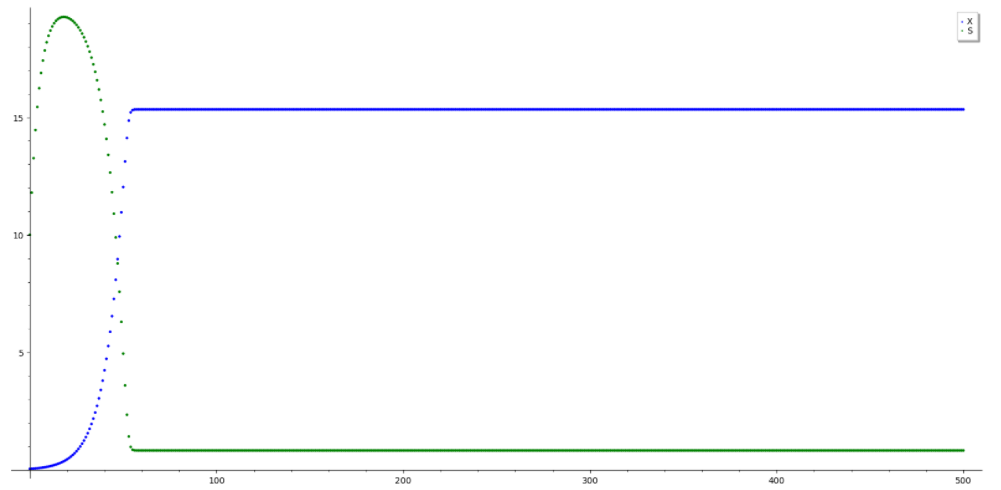
\includegraphics[scale=0.5]{Modelo_12.png}} 
        \caption*{Diminuindo a constante de saturação pela metade (12)}
\end{figure}
\vspace{-7mm}
\begin{itemize}
\begin{multicols}{4}
    \item $\mu_{max} = 1.6$ 
    \item $K_s = 0.5$ 
\columnbreak    
    \item $Y = 0.8$ 
    \item $S_f = 20$ 
\columnbreak    
    \item $D = 1.0$ 
    \item $X_0 = 0.05$ 
\columnbreak    
    \item $S_0 = 10.0$ 
    \item $\mu = 1.0$
\end{multicols}
\end{itemize} 
%FEITO 8
\begin{figure}[H]
        \centering
        \hbox{\hspace{1.0em} 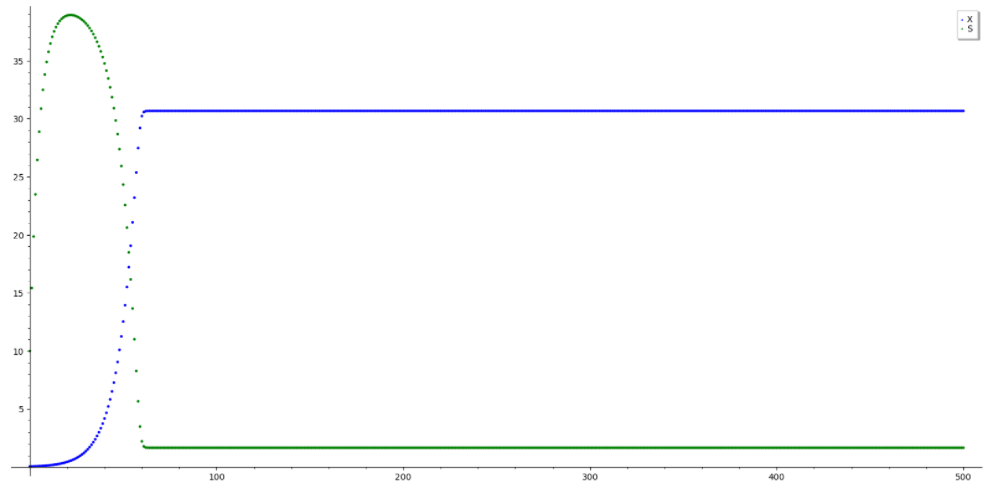
\includegraphics[scale=0.5]{Modelo_13.png}} 
        \caption*{Dobrando o limite de concentração de entrada do substrato (13)}
\end{figure}
\vspace{-7mm}
\begin{itemize}
\begin{multicols}{4}
    \item $\mu_{max} = 1.6$ 
    \item $K_s = 1.0$ 
\columnbreak    
    \item $Y = 0.8$ 
    \item $S_f = 40$ 
\columnbreak    
    \item $D = 1.0$ 
    \item $X_0 = 0.05$ 
\columnbreak    
    \item $S_0 = 10.0$ 
    \item $\mu = 1.0$
\end{multicols}
\end{itemize} 
%FEITO 9 
\begin{figure}[H]
        \centering
        \hbox{\hspace{1.0em} 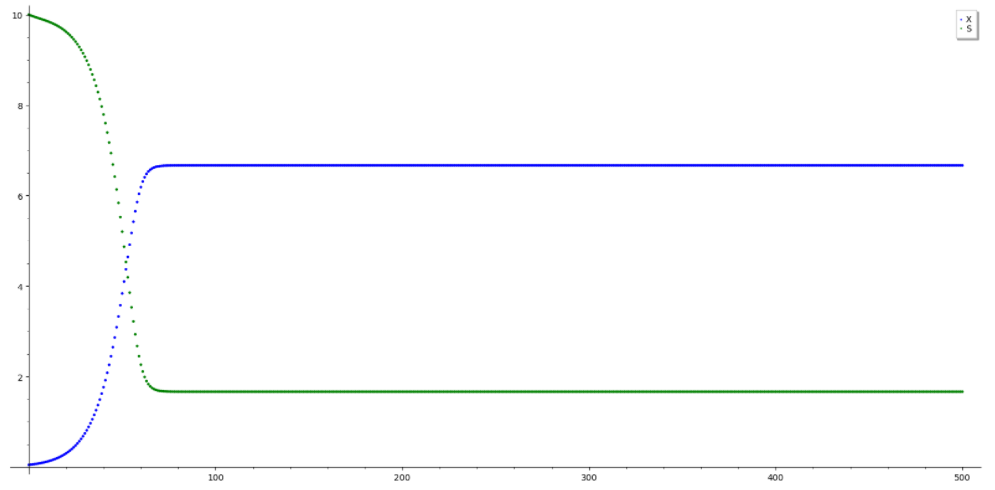
\includegraphics[scale=0.5]{Modelo_14.png}} 
        \caption*{Diminuindo o limite de concentração de entrada do substrato pela metade (14)}
\end{figure}
\vspace{-7mm}
\begin{itemize}
\begin{multicols}{4}
    \item $\mu_{max} = 1.6$ 
    \item $K_s = 1.0$ 
\columnbreak    
    \item $Y = 0.8$ 
    \item $S_f = 10$ 
\columnbreak    
    \item $D = 1.0$ 
    \item $X_0 = 0.05$ 
\columnbreak    
    \item $S_0 = 10.0$ 
    \item $\mu = 1.0$
\end{multicols}
\end{itemize} 
%FEITO 10
\begin{figure}[H]
        \centering
        \hbox{\hspace{1.0em} 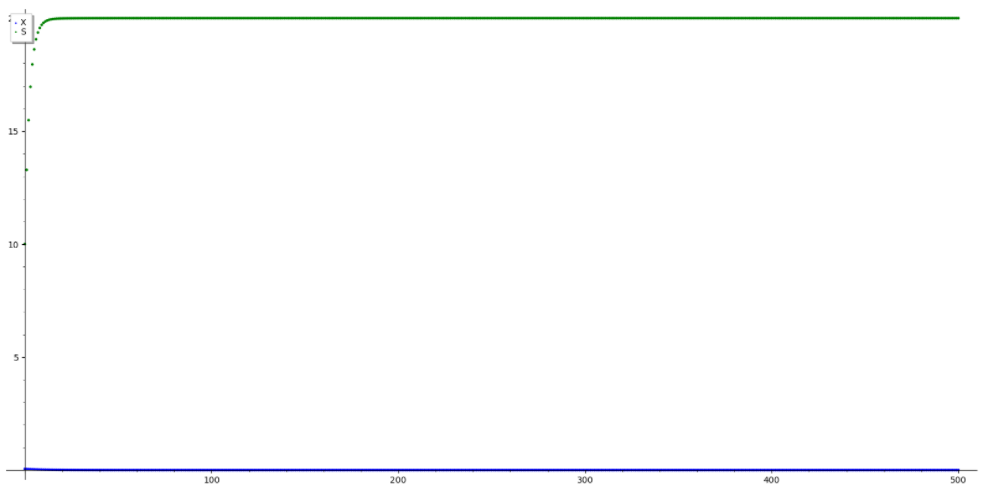
\includegraphics[scale=0.5]{Modelo_15.png}} 
        \caption*{Dobrando a taxa de diluição (15)}
\end{figure}
\vspace{-7mm}
\begin{itemize}
\begin{multicols}{4}
    \item $\mu_{max} = 1.6$ 
    \item $K_s = 1.0$ 
\columnbreak    
    \item $Y = 0.8$ 
    \item $S_f = 20$ 
\columnbreak    
    \item $D = 2.0$ 
    \item $X_0 = 0.05$ 
\columnbreak    
    \item $S_0 = 10.0$ 
    \item $\mu = 2.0$
\end{multicols}
\end{itemize} 
%FEITO 11
\begin{figure}[H]
        \centering
        \hbox{\hspace{1.0em} 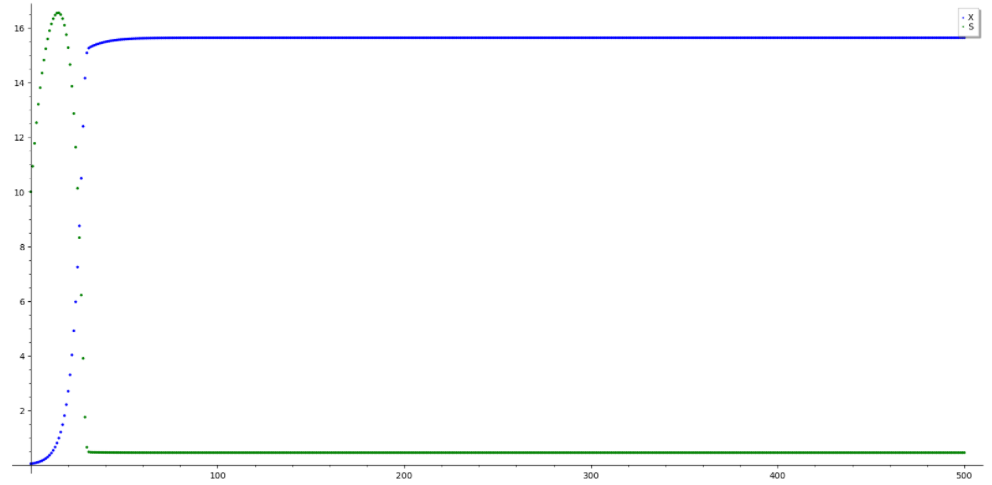
\includegraphics[scale=0.5]{Modelo_16.png}} 
        \caption*{Diminuindo a taxa de diluição pela metade (16)}
\end{figure}
\vspace{-7mm}
\begin{itemize}
\begin{multicols}{4}
    \item $\mu_{max} = 1.6$ 
    \item $K_s = 1.0$ 
\columnbreak    
    \item $Y = 0.8$ 
    \item $S_f = 20$ 
\columnbreak    
    \item $D = 0.5$ 
    \item $X_0 = 0.05$ 
\columnbreak    
    \item $S_0 = 10.0$ 
    \item $\mu = 0.5$
\end{multicols}
\end{itemize} 
%FEITO 13
\begin{figure}[H]
        \centering
        \hbox{\hspace{1.0em} 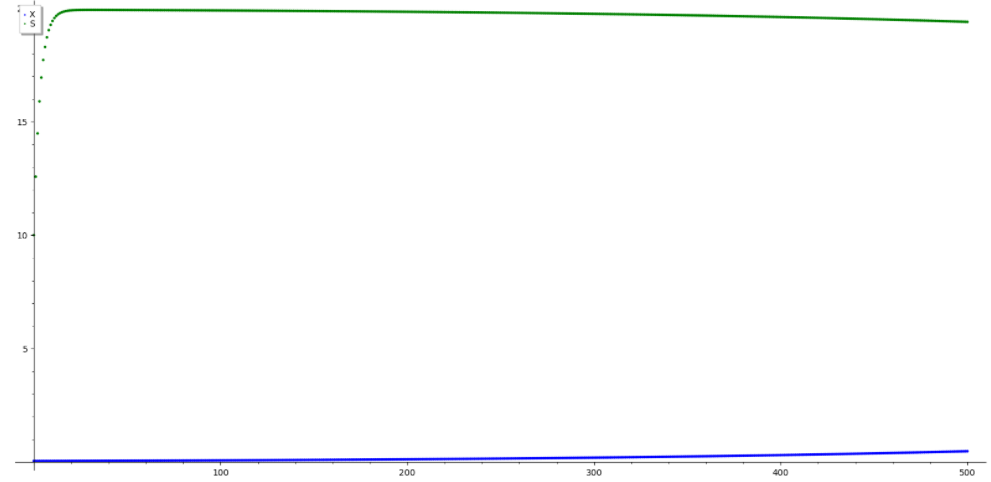
\includegraphics[scale=0.5]{Modelo_17.png}} 
        \caption*{Aumentando a taxa de diluição (17)}
\end{figure}
\vspace{-7mm}
\begin{itemize}
\begin{multicols}{4}
    \item $\mu_{max} = 1.6$ 
    \item $K_s = 1.0$ 
\columnbreak    
    \item $Y = 0.8$ 
    \item $S_f = 20$ 
\columnbreak    
    \item $D = 1.5$ 
    \item $X_0 = 0.05$ 
\columnbreak    
    \item $S_0 = 10.0$ 
    \item $\mu = 1.5$
\end{multicols}
\end{itemize}
%FEITO 14

\begin{figure}[h]
\centering
    \begin{subfigure}
         
         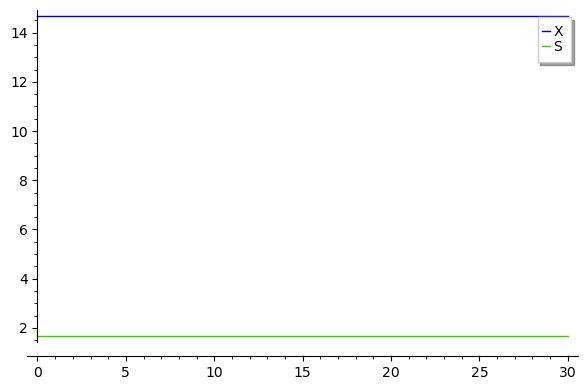
\includegraphics[scale = 0.4]{equim/eq1.png}
         \caption*{Parâmetros originais (1*)}
\begin{itemize}
\begin{multicols}{4}
    \item $\mu_{max} = 1.6$ 
    \item $K_s = 1.0$ 
\columnbreak     
    \item $Y = 0.8$ 
    \item $S_f = 20$ 
\columnbreak    
    \item $D = 1.0$ 
    \item $X_0 = 0.05$ 
\columnbreak     
    \item $S_0 = 10.0$ 
    \item $\mu = 1.0$
\end{multicols}
\end{itemize} 
    \end{subfigure}

\begin{subfigure}

     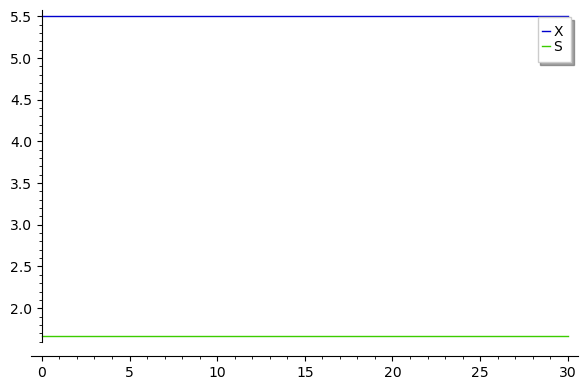
\includegraphics[scale= 0.4]{equim/eq2.png}
     \caption*{Diminuindo o coeficiente de rendimento (2*)}
\begin{itemize}
\begin{multicols}{4}
    \item $\mu_{max} = 1.6$ 
    \item $K_s = 1.0$ 
\columnbreak     
    \item $Y = 0.3$ 
    \item $S_f = 20$ 
\columnbreak    
    \item $D = 1.0$ 
    \item $X_0 = 0.05$ 
\columnbreak     
    \item $S_0 = 10.0$ 
    \item $\mu = 1.0$
\end{multicols}
\end{itemize} 
\end{subfigure}
\end{figure}
\newpage
\begin{figure}[!h]
\centering
     \begin{subfigure}
         
         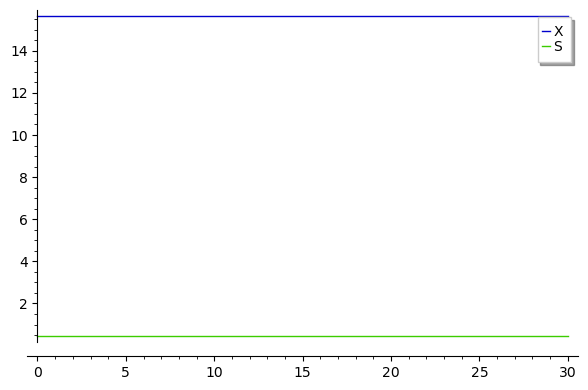
\includegraphics[scale = 0.5]{equim/eq3.png}
         \caption*{Dobrando a taxa máxima de crescimento (3*)}
        \begin{itemize}
\begin{multicols}{4}
    \item $\mu_{max} = 3.2$ 
    \item $K_s = 1.0$ 
\columnbreak     
    \item $Y = 0.8$ 
    \item $S_f = 20$ 
\columnbreak    
    \item $D = 1.0$ 
    \item $X_0 = 0.05$ 
\columnbreak     
    \item $S_0 = 10.0$ 
    \item $\mu = 1.0$
\end{multicols}
\end{itemize} 
\end{subfigure}

    \begin{subfigure}
         
         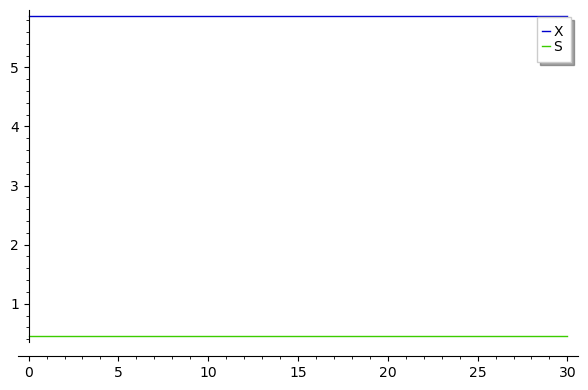
\includegraphics[scale = 0.5]{equim/eq4.png}
         \caption*{Dobrando a taxa máxima de crescimento e diminuindo o coeficiente de rendimento (4*)}
                \begin{itemize}
        \begin{multicols}{4}
            \item $\mu_{max} = 3.2$ 
            \item $K_s = 1.0$ 
        \columnbreak    
            \item $Y = 0.3$ 
            \item $S_f = 20$ 
        \columnbreak    
            \item $D = 1.0$ 
            \item $X_0 = 0.05$ 
        \columnbreak    
            \item $S_0 = 10.0$ 
            \item $\mu = 1.0$
        \end{multicols}
        \end{itemize} 
    \end{subfigure}

\begin{subfigure}
     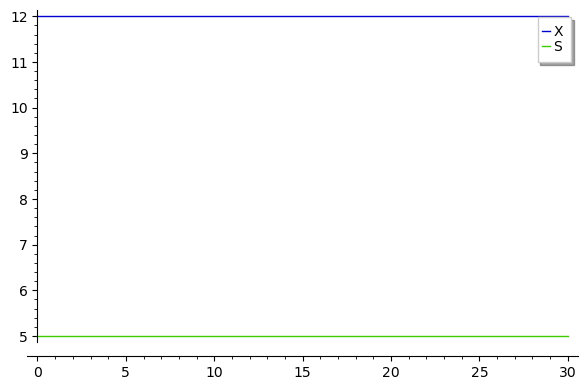
\includegraphics[scale= 0.5]{equim/eq5.png}
     \caption*{Diminuindo a taxa máxima de crescimento (5*)}
     \begin{itemize}
\begin{multicols}{4}
    \item $\mu_{max} = 1.2$ 
    \item $K_s = 1.0$ 
\columnbreak    
    \item $Y = 0.8$ 
    \item $S_f = 20$ 
\columnbreak    
    \item $D = 1.0$ 
    \item $X_0 = 0.05$ 
\columnbreak    
    \item $S_0 = 10.0$ 
    \item $\mu = 1.0$
\end{multicols}
\end{itemize}
\end{subfigure}
\end{figure}
\newpage
\begin{figure}[!h]
\centering
     \begin{subfigure}
         
         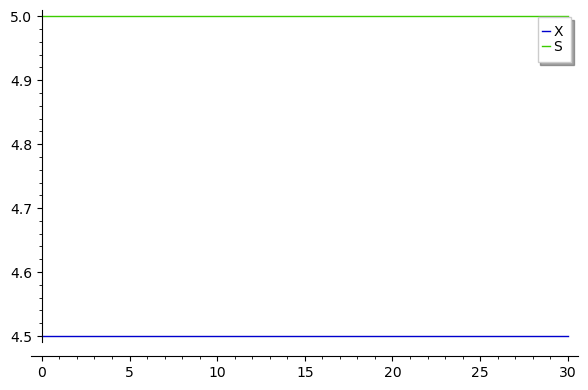
\includegraphics[scale = 0.5]{equim/eq6.png}
         \caption*{Diminuindo a taxa máxima de crescimento e diminuindo o coeficiente de rendimento (6*)}
 \begin{itemize}
\begin{multicols}{4}
    \item $\mu_{max} = 1.2$ 
    \item $K_s = 1.0$ 
\columnbreak    
    \item $Y = 0.3$ 
    \item $S_f = 20$ 
\columnbreak    
    \item $D = 1.0$ 
    \item $X_0 = 0.05$ 
\columnbreak    
    \item $S_0 = 10.0$ 
    \item $\mu = 1.0$
\end{multicols}
\end{itemize} 
\end{subfigure}

    \begin{subfigure}
         
         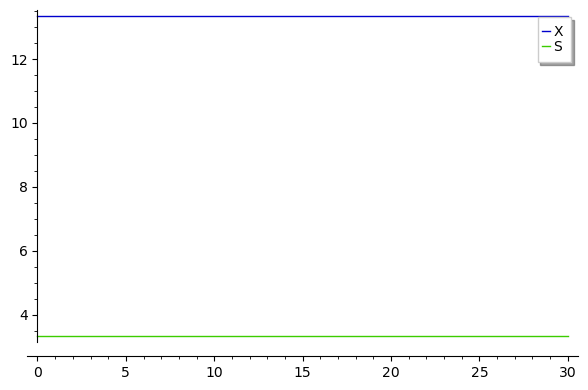
\includegraphics[scale = 0.5]{equim/eq7.png}
         \caption*{Dobrando a constante de saturação (11*)}
\begin{itemize}
\begin{multicols}{4}
    \item $\mu_{max} = 1.6$ 
    \item $K_s = 2.0$ 
\columnbreak    
    \item $Y = 0.8$ 
    \item $S_f = 20$ 
\columnbreak    
    \item $D = 1.0$ 
    \item $X_0 = 0.05$ 
\columnbreak    
    \item $S_0 = 10.0$ 
    \item $\mu = 1.0$
\end{multicols}
\end{itemize} 
    \end{subfigure}

\begin{subfigure}
     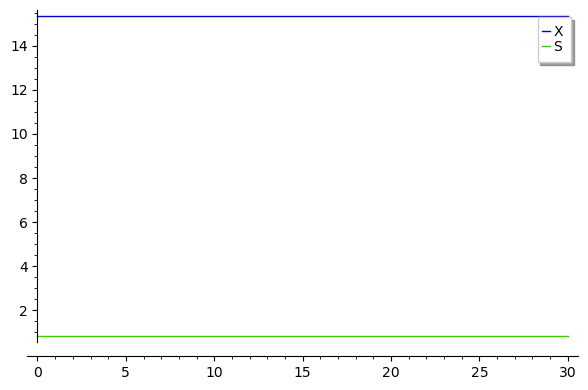
\includegraphics[scale= 0.5]{equim/eq8.png}
     \caption*{Diminuindo a constante de saturação pela metade (12*)}
\begin{itemize}
\begin{multicols}{4}
    \item $\mu_{max} = 1.6$ 
    \item $K_s = 0.5$ 
\columnbreak    
    \item $Y = 0.8$ 
    \item $S_f = 20$ 
\columnbreak    
    \item $D = 1.0$ 
    \item $X_0 = 0.05$ 
\columnbreak    
    \item $S_0 = 10.0$ 
    \item $\mu = 1.0$
\end{multicols}
\end{itemize} 
\end{subfigure}
\end{figure}

\newpage

\begin{figure}[!h]
\centering
     \begin{subfigure}
         
         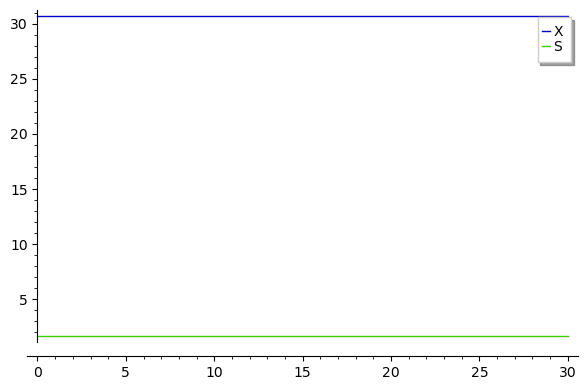
\includegraphics[scale = 0.5]{equim/eq9.png}
         \caption*{Dobrando o limite de concentração de entrada do substrato (13*)}
\begin{itemize}
\begin{multicols}{4}
    \item $\mu_{max} = 1.6$ 
    \item $K_s = 1.0$ 
\columnbreak    
    \item $Y = 0.8$ 
    \item $S_f = 40$ 
\columnbreak    
    \item $D = 1.0$ 
    \item $X_0 = 0.05$ 
\columnbreak    
    \item $S_0 = 10.0$ 
    \item $\mu = 1.0$
\end{multicols}
\end{itemize}  
\end{subfigure}

    \begin{subfigure}
         
         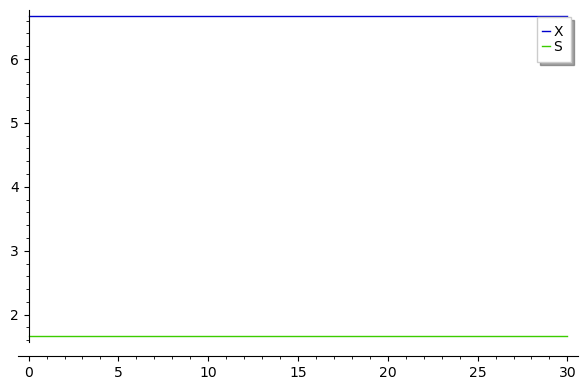
\includegraphics[scale = 0.5]{equim/eq10.png}
         \caption*{Diminuindo o limite de concentração de entrada do substrato pela metade (14*)}
\begin{itemize}
\begin{multicols}{4}
    \item $\mu_{max} = 1.6$ 
    \item $K_s = 1.0$ 
\columnbreak    
    \item $Y = 0.8$ 
    \item $S_f = 10$ 
\columnbreak    
    \item $D = 1.0$ 
    \item $X_0 = 0.05$ 
\columnbreak    
    \item $S_0 = 10.0$ 
    \item $\mu = 1.0$
\end{multicols}
\end{itemize} 
    \end{subfigure}

\begin{subfigure}
     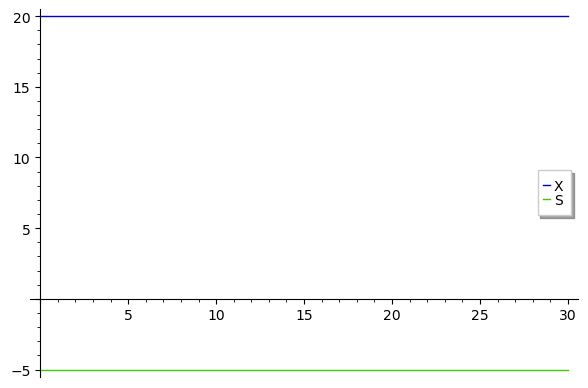
\includegraphics[scale= 0.5]{equim/eq11.png}
     \caption*{Dobrando a taxa de diluição (15*)}
\begin{itemize}
\begin{multicols}{4}
    \item $\mu_{max} = 1.6$ 
    \item $K_s = 1.0$ 
\columnbreak    
    \item $Y = 0.8$ 
    \item $S_f = 20$ 
\columnbreak    
    \item $D = 2.0$ 
    \item $X_0 = 0.05$ 
\columnbreak    
    \item $S_0 = 10.0$ 
    \item $\mu = 2.0$
\end{multicols}
\end{itemize} 
\end{subfigure}
\end{figure}
\newpage
\begin{figure}[!    h]
\centering
    \begin{subfigure}
         
         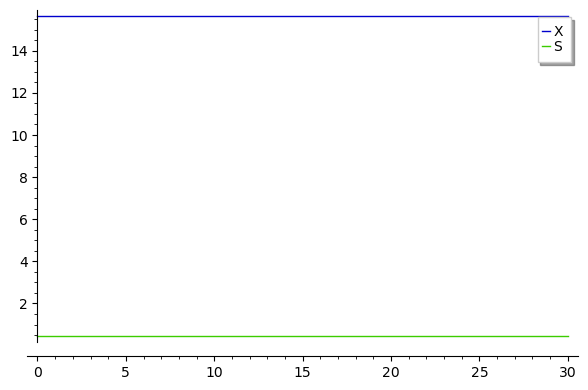
\includegraphics[scale = 0.5]{equim/eq13.png}
         \caption*{Diminuindo a taxa de diluição pela metade (16*)}
\begin{itemize}
\begin{multicols}{4}
    \item $\mu_{max} = 1.6$ 
    \item $K_s = 1.0$ 
\columnbreak    
    \item $Y = 0.8$ 
    \item $S_f = 20$ 
\columnbreak    
    \item $D = 0.5$ 
    \item $X_0 = 0.05$ 
\columnbreak    
    \item $S_0 = 10.0$ 
    \item $\mu = 0.5$
\end{multicols}
\end{itemize} 
    \end{subfigure}

\begin{subfigure}
     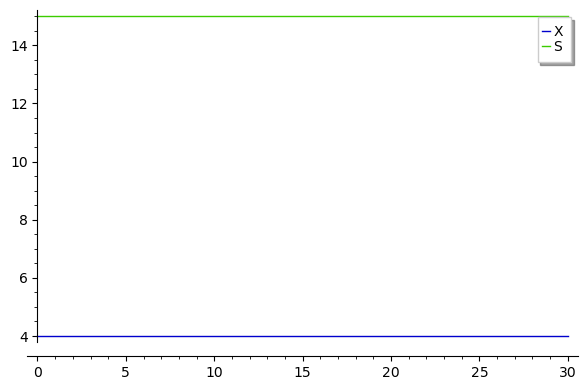
\includegraphics[scale= 0.5]{equim/eq14.png}
     \caption*{Aumentando a taxa de diluição (17*)}
\begin{itemize}
\begin{multicols}{4}
    \item $\mu_{max} = 1.6$ 
    \item $K_s = 1.0$ 
\columnbreak    
    \item $Y = 0.8$ 
    \item $S_f = 20$ 
\columnbreak    
    \item $D = 2.0$ 
    \item $X_0 = 0.05$ 
\columnbreak    
    \item $S_0 = 10.0$ 
    \item $\mu = 2.0$
\end{multicols}
\end{itemize} 
\end{subfigure}
\end{figure}

\newpage
\\\\\textbf{Relembrando as fórmulas:}
\begin{center}
    $(dX/dt) &= \mu X-DX$     
  \\$(dS/dt) &= DS_f-DS-(\mu X/Y)$
  \\$\mu &= \mu_{max}S/(K_s+S)$
  \\$X_{Eq} &= Y(S_f - \frac{DK_s}{\mu_{max}-D})$
  \\$S_{Eq} &= \frac{K_sD}{\mu_{max}-D}$
\end{center}
\\\\
\textbf{\Large{Discussão}}
\\\\Agora que temos todos os gráficos plotados, podemos analisá-los.
\\\\Em geral, é notável que os gráficos têm um formato bem similar, com a taxa de concentração celular ($X$) crescente ao longo do tempo, até se estabilizar, e a taxa limite de concentração do substrato de saída ($S$) formando uma parábola, quase sempre extremamente próxima do eixo y, e que rapidamente decai e se estabiliza próxima de 0.
\\\\Analisando agora os resultados entre si, é possível ver que, usando os valores de parâmetros encontrados em $^{[20]}$ ($\mu_{max} = 1.6, K_s = 1.0, Y = 0.8, S_f = 20.0$ e $D = 1.0$), alterar o coeficiente de rendimento $Y$, mais especificamente diminuí-lo, faz com que a concentração celular aumente muito menos em comparação com o valor original do parâmetro, já que $Y$ afeta positivamente $X$, e nesse caso, $Y$ está menor do que seu valor original. O limite de concentração de saída do substrato parece menos afetado, apenas tendo o comprimento de sua curva um pouco menor, já que diminuir o denominador aumenta o valor da fração negativa, enquanto que seu nível de estabilidade é o mesmo em ambos os casos, já que $Y$ não afeta o equilíbrio de $S$. Isso pode visto entre (1) e (2) e (1*) e (2*).
\\\\Dobrando a taxa máxima de crescimento $\mu_{max}$, é notável que $X$ sobe muito mais rapidamente, já que $\mu_{max}$ afeta positivamente esse parâmetro por estar no denominador de uma fração negativa, enquanto que $S$ decai tão rápido quanto, já que aumentar $\mu_{max}$ significa diminuir o valor da fração. O equilíbrio de $X$ também é positivamente afetado, estando agora mais próximo de 16 do que de 15, enquanto $S$ está muito mais próximo de 0. Diminuindo $Y$ com $\mu_{max}$ dobrado é possível observar um efeito similar ao que aconteceu anteriormente, com $X$ subindo muito menos e a curva de $S$ decaindo um pouco antes. Isso pode ser visto comparando a integração e equilíbrio dos 4 primeiros gráficos. 
\\\\Diminuindo a taxa máxima de crescimento temos um retardo na chegada ao equilíbrio. Era o esperado, já que a concentração de substrato vai diminuir de forma mais lenta por conta do crescimento não tão acelerado da concentração de massa celular, como pode ser visto no gráfico (5). Ao combinarmos a diminuição da taxa máxima de crescimento com a diminuição do coeficiente de rendimento (6), obtivemos um crescimento muito menor da concentração de massa celular, algo que também é esperado já que com a mesma quantidade de substrato que tinhamos no equilíbrio de (5) teremos agora um rendimento menor, que afeta a reprodução dos microorganismos negativamente.
\\\\Nos testes em que foram mudadas apenas as condições iniciais ($X_0$ e $S_0$), percebe-se que não há mudança no nível de estabilidade, já que $X$ e $S$ não afetam o próprio sistema de equilíbrio. Portanto, não plotamos os gráficos com os equilíbrios para as situações mostradas em (7), (8), (9) e (10), já que o equilíbrio seria o mesmo de (1), como observado. Além disso, é claro que alterar as taxas iniciais alteraria o gráfico apenas por modificar o valor inicial deles.
\\\\Dobrar a constante de saturação $K_s$ acaba por diminuir a diferença entre os estados estacionários, já que enquanto esse parâmetro afeta positivamente o equilíbrio de $S$, ele afeta negativamente o de $X$. Como consequência, diminuir essa taxa pela metade leva a um aumento na diferença entre os estados, levando $S$ a se aproximar muito de 0 e $X$ se aproximar mais de 15. Por interferir negativamente em $dX/dt$ e positivamente em $dS/dt$, é possível notar também a diferença que $K_s$ exerce no comprimento da onda de $S$ e na velocidade de $X$ para atingir seu equilíbrio. Isso pode ser visto entre os gráficos (11) e (12) e (11*) e (12*). 
\\\\ Diminuir o limite de concentração de entrada do substrato leva a uma diferença menor entre o nível dos estados estacionários se comparado a diminuição de saída do substrato (14) e (14*), enquanto que dobrar o limite de entrada aumenta a diferença se comparado ao aumento do substrato de saída (13) e (13*). Também há uma diferença notável entre eles, já que $S_f$ está diretamente relacionado com X: se $S_f$ aumenta, o valor de X aumenta e vice-versa.
\\\\Alterando os parâmetros da diluição, encontramos nosso primeiro resultado problemático do trabalho. Isso pode ser visto nos gráficos (15) e (15*), onde em 15 $S$ sobe até se aproximar de 20, enquanto $X$ decai e se aproxima de 0. Por outro lado, o gráfico dos equilíbrios apresenta resultados distintos, com $X$ em 20 e $S$ negativo. Apesar do resultado problemático, sabemos o porquê dele: $D$ deve ser menor ou igual a $\frac{\mu_{max}S_f}{K_s+S_f}$, e nesse caso, onde $\mu_{max} = 1.6, S_f = 20$ e $K_s = 1.0$, $D$ deveria ser menor que $\frac{32}{21} = 1.52380952$. Por conta disso, como o valor de $D$ passado foi maior que 1.52, no caso 2.0, o modelo não foi capaz de ser executado corretamente. 
\\\\Diminuindo a taxa de diluição pela metade ((16) e (16*)), o gráfico volta a se assemelhar aos demais. É possível notar que a concentração de substrato chega a um pico menor que pela taxa original, e decai até o estado estacionário em praticamente metade do tempo original, enquanto que a concentração celular também chega a seu estado estacionário de forma bem mais rápida, mas atinge um nível similar ao original. 
\\\\Para analisar melhor a limitação da taxa $D$ citada anteriormente, deixamos ela sutilmente menor que o seu limite, passando o valor 1.5 para ela, e é possível notar que o gráfico também é bem afetado por isso: devido ao "alto" valor da taxa, o gráfico (17) se assemelha ao (15), todavia, estudando o gráfico (17*), é notável que os valores de equilíbrio fazem mais sentido que os encontrados em (15*). Por isso, dá pra se imaginar que, aumentando a faixa de tempo de análise do modelo, o gráfico fique mais semelhante aos outros.
\\\\
\textbf{\Large{Conclusão}}
\\\\Analisando todos os resultados que obtivemos estudando o modelo mais simples de Monod, é possível afirmar que ele ainda pode ser considerado válido para uso em estudo mais amplo sobre o ambiente do quimiostato. Como utilizamos um único tipo celular não especificado, usar um coeficiente de biomassa constante não causou interferências visíveis no quesito de oscilações no sistema. Por essa razão, também não foi necessário fazer uso de um modelo tridimensional para atingir a estabilidade.
\\\\Apesar disso, no caso de um estudo mais avançado sobre o ambiente do quimiostato, que lide com dados reais, de fato seria necessário fazer as adaptações recomendadas na introdução desse artigo. Entre eles, deveria ser considerado o atraso no ajuste da taxa específica de crescimento, $\mu$, que seria feito utilizando equações diferenciais parciais de atraso, o que não se encaixa nesse trabalho no período atual do curso, dado que ainda não estudamos $EDPs$. 

\newpage

\begin{thebibliography}{9}
\\\\
\bibitem{relatorio} 
Wikipedia. 
\\
\textit{Chemostat}. 
\\\texttt{https://en.wikipedia.org/wiki/Chemostat}
\\\\
\bibitem{relatorio2}
ScienceDirect.
\\
\textit{Chemostat}
\\\texttt{https://www.sciencedirect.com/topics/earth-and-planetary-sciences/chemostat}
\\\\
\bibitem{relatorio3}
The Chemostat (Volume 1).
\\
\textit{Mathematical Theory of Microorganism Cultures. 2017.}
\\\texttt{https://books.google.com.br/books?hl=pt-BR\&lr=\&id=e4MtDwAAQBAJ\&oi=fnd\&pg=PP2\&dq=mathematical
\\+chemostat\&ots=yqWBX1qPGP\&sig=f8-\_BXxMKAB8-E6h8td66ONpr\_M\#v=onepage\&q=mathematical$\%$20chemostat
\\ \&f=false}
\\\\
\bibitem{relatorio4}
Naomi Ziv, Nathan J. Brandt e David Gresham. 2013
\\
\textit{Journal of Visualized Experiments}.
\textit{The Use of Chemostats in Microbial Systems Biology}.
\\\texttt{https://www.ncbi.nlm.nih.gov/pmc/articles/PMC3940325/pdf/jove-80-50168.pdf}
\\\\
\bibitem{relatorio5}
S. M. Sohel Rana and Ummi Kulsum. 2012.
\\
\textit{A Mathematical Model Related To Chemostat With Variable Yields}.
\textit{Department of Mathematics, University of Dhaka, Dhaka-1000, Bangladesh}.
\textit{Dhaka Univ. J. Sci. 60(2): 147-152, 2012}
\\\texttt{https://www.banglajol.info/index.php/DUJS/article/view/11482}
\\\\
\bibitem{relatorio6}
Jean-Luc Gouzé, Valérie Lemesle. 2008.
\\
\textit{Two simple growth models in the chemostat.}
\\\texttt{https://hal.inria.fr/hal-01277831/document}
\\\\
\bibitem{relatorio7}
Porro et. al. 1988.
\\
\textit{Oscillations in continuous cultures of budding yeast: a segregated parameter analysis.}
\\\texttt{https://pubmed.ncbi.nlm.nih.gov/18587737/}
\\\\
\bibitem{relatorio8}
R. Nisbet and W. Gurney. 1982.
\\
\textit{Modelling Fluctuating Populations.}
\\\texttt{https://www.amazon.com/Modelling-Fluctuating-Populations-R-Nisbet/dp/1930665903}
\\\\
\bibitem{relatorio9}
Zhu, L. and X.C. Huang. 2005.
\\
\textit{Relative positions of limit cycles in a continuous culture vessel with variable yields}.
\textit{Journal of Mathematical Chemistry, 38, 2:119-128.}
\\
\textit{Multiple limit cycles in a continuous culture vessel Nonlinear analysis: Theory, Methods and Applications.}
\\\\
\bibitem{relatorio10}
Pilyugin S. S. and P. Waltman, 2003. 
\\
\textit{Multiple limit cycles in the chemostat with variable yield, Math. Biosci. 182, 151-166.}
\\\\
\bibitem{relatorio11}
Song G. and X. Li, 1999. 
\\
\textit{Stability of solution to the chemostat system with non-constant consuming rate, J. Biomath. 14:1, 24.}
\\\\
\bibitem{relatorio12}
Wikipedia.
\\
\textit{Monod equation}.
\\\texttt{https://en.wikipedia.org/wiki/Monod\_equation}.
\\\\
\bibitem{relatorio13}
T. B. Young, D. F. Bruley, e H. R. Bungay. 1970.
\\
\textit{A dynamic mathematical model of the chemostat}
\textit{Clemson University, Clemson, South Carolina 29631}
\\\texttt{https://onlinelibrary.wiley.com/doi/abs/10.1002/bit.260120506}
\\\\
\bibitem{relatorio14}
Wikipedia. 
\\
\textit{Histerese}. 
\\\texttt{https://pt.wikipedia.org/wiki/Histerese}
\\\\
\bibitem{relatorio15}
LAASP. 
\\
\textit{What's Hysteresis?}. 
\\\texttt{https://www.lassp.cornell.edu/sethna/hysteresis/WhatIsHysteresis.html}
\\\\
\bibitem{relatorio16}
R. I. Mateles, D. Y. Ryu, and T. Yasuda, Nature, 208,263 (1965). 
\\
\textit{Measurement of Unsteady State Growth Rates of Micro-Organisms}. 
\\\texttt{https://www.nature.com/articles/208263a0}
\\\\
\bibitem{relatorio17}
F. F. Storer and A. F. Gaudy, Environ. Sci. Technol., 3, 143 (1969). 
\\
\textit{Computational analysis of transient response to quantitative shock loadings of heterogeneous populations in continuous culture}. 
\\\texttt{https://pubs.acs.org/doi/10.1021/es60025a007}
\\\\
\bibitem{relatorio18}
Engineering LibreTexts. 
\\
\textit{Bacterial Chemostat}. 
\\\texttt{https://eng.libretexts.org/Bookshelves/Industrial\_and\_Systems\_Engineering/Book$\%$3A\_Chemical\_Process
\\\_Dynamics\_and\_Controls\_(Woolf)/06$\%$3A\_Modeling\_Case\_Studies/6.03$\%$3A\_Bacterial\_Chemostat}
\\\\
\bibitem{relatorio19}
The continuous culture of bacteria.
\\\texttt{HERBERT D, ELSWORTH R, TELLING RC. The continuous culture of bacteria; a theoretical and experimental study. J Gen Microbiol. 1956 Jul;14(3):601-22. doi: 10.1099/00221287-14-3-601. PMID: 13346021.}
\\\\
\bibitem{relatorio20}
Analytical solution for a hybrid Logistic-Monod cell growth model in batch and continuous stirred tank reactor culture.
\\
\textit{Xu P. Analytical solution for a hybrid Logistic‐Monod cell growth model in batch and continuous stirred tank reactor culture. Biotechnology and Bioengineering. 2020;117:873–878.}
\\\texttt{https://doi.org/10.1002/bit.27230}
\\\\
\bibitem{relatorio21}
Analyses of various control schemes for continuous bioreactors
\\
\textit{Pramod AgrawalHenry C. Lim. 2005}
\\\texttt{https://link.springer.com/chapter/10.1007/BFb0006380}
\\\\
\bibitem{relatorio22}
Analisando a Estabilidade de Equilíbrios.
\\Repositório Principal: \textit{fccoelho/Modelagem-Matematica-IV} (\texttt{https://github.com/fccoelho/
\\Modelagem-Matematica-IV}). 
\\\textit{Aula 1 - Analizando EDOs}
\\(\texttt{https://github.com/fccoelho/Modelagem-Matematica-IV/blob/master/Planilhas\%20Sage/
\\Aula\%201\%20-\%20Analizando\%20EDOs.ipynb}).
\\\textit{Aula 3 - Análise de Estabilidade Linear} 
\\(\texttt{https://github.com/fccoelho/Modelagem-Matematica-IV/blob/master/Planilhas\%20Sage/
\\Aula\%203\%20-\%20An\%C3\%A1lise\%20de\%20Estabilidade\%20Linear.ipynb}).
\\\\
\bibitem{relatorio23}
Notebooks de base para modelagem.
\\Repositório Principal: \textit{jckantor/CBE30338} (\texttt{https://github.com/jckantor/CBE30338}). 
\\\textit{2.4 Continuous Product Blending} 
\\(\texttt{https://jckantor.github.io/CBE30338/02.04-Continuous-Product-Blending.html}).
\\\textit{2.7 Fed-Batch Bioreactor} 
\\(\texttt{https://jckantor.github.io/CBE30338/02.07-Fed-Batch-Bioreactor.html}).
\\\\
\bibitem{relatorio24}
University of Oregon.
\\
\textit{Eigenvectors and eigenvalues in Sage}
\\\texttt{https://blogs.uoregon.edu/math342sp16lipshitz/sample-page/eigenvectors-and-eigenvalues-in-sage/}
\\\\



\end{thebibliography} 


\end{document}